%%%%%%%%%%%%%%%%%%%%%%%%%%%%%%%%%%%%%%%%%%%%%%%%%%%%%%%%%%%%%%%%%%%%%%%%%%%%%%%%
% simulation.tex: Chapter on MC production:
%%%%%%%%%%%%%%%%%%%%%%%%%%%%%%%%%%%%%%%%%%%%%%%%%%%%%%%%%%%%%%%%%%%%%%%%%%%%%%%%
\chapter{Simulation}
\label{chapter:ldmx:simulation}
%%%%%%%%%%%%%%%%%%%%%%%%%%%%%%%%%%%%%%%%%%%%%%%%%%%%%%%%%%%%%%%%%%%%%%%%%%%%%%%%

\ac{ldmx} (like many other HEP experiments) uses an intricate software stack in order to realistically and efficiently simulate particle interactions with the detector, emulate the electronics that would be used to measure these interactions, and reconstruct the output of these electronics into physically-understandable variables.
These software tasks are accomplished by a wide swath of different software packages, some of which custom-written for \ac{ldmx}, most of which written in C++.
This chapter is focused on describing this simulation infrastructure -- focusing particularly on parts of the infrastructure I was involved in -- while also pointing out areas that are expected to remain constant in the presence of data gathered from a real detector.
After a discussion of general data processing, I move into discussing the specific samples
used to do this simulation study.

\section{General Data Process}
One of the core principles helping organize HEP data is the concept of an ``event.'' In the context
of \ac{ldmx}, an event is the data collected within a small window of time around the arrival of a
beam electron into our detector apparatus. In essence, each event within the software is
independent from one another however they all share a similar structure to the information they
hold. A natural example is a data table: a row has the same values in each of its columns as all
the other rows. Events behave the same way; however, unlike a data table, the structure of an event
can be more intricate than simply a series of values corresponding to different column titles.
While our basic ``unit'' of data is an event, we require many events in order to make statistical
conclusions about our data; thus, we have developed an ``event processing framework'' that allows
us to unify the various aspects of processing the data held within an event.

\begin{figure}
  \centering
  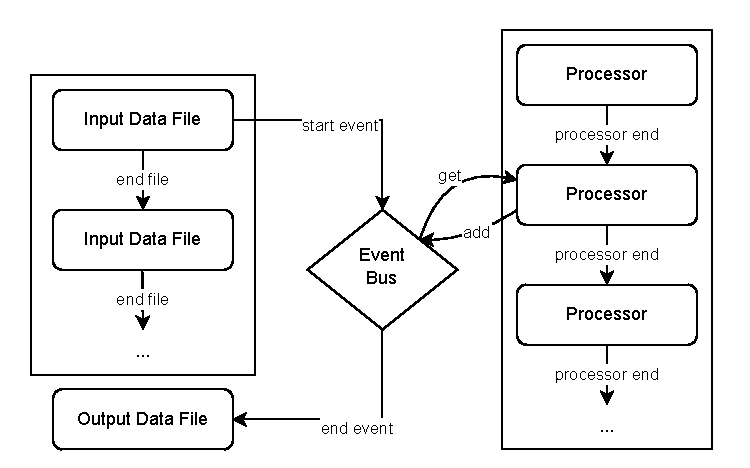
\includegraphics[width=0.9\textwidth]{figures/ldmx/simulation/FrameworkFlowChart.drawio.pdf}
  \caption{Flow chart of how data is processed in the \ac{ldmx} framework. Each processor has the ability to ``add" data to the event as well as ``get" data from the event. The processors are run in a user-defined sequence. Data can also be loaded from one or more input data files where the event data from those files is loaded into memory before the first processor is run. After all processors are done with an event, it is saved to the output data file.}
  \label{fig:ldmx:sim:data-flow}
\end{figure}

The event processing framework designed, developed, and maintained by \ac{ldmx} is designed to
allow the flexibility necessary to do the wide range of tasks necessary for the experiment. The C++
framework uses CERN's ROOT \cite{cernroot} for data serialization, Boost \todo[citation]{need a
  citaiton for Boost libraries} for logging, and Python \cite{python} for dynamic run-time
configuration. As diagramed in \cref{fig:ldmx:sim:data-flow}, the design is a sequential model: the
``event bus" stops at the individual processors in a certain sequence. The individual processors
can inspect the data currently on the bus and board more passengers onto the bus for later
processors to use and which are eventually serialized into the output ROOT file. The processors can
be built separately from the framework and then dynamically loaded and created at run-time by an
abstract factory. This design choice allows for all of the computationally-intensive software tasks
necessary for \ac{ldmx} (simulation, reconstruction and some analysis tasks) to use this framework
and be organized into separate modules which are only loaded into memory when that module is being
used.

The serialization portion of the framework is similarly dynamic; focusing on enabling users' code
to add data structures from the most simple (e.g. individual booleans) to the most complicated
(e.g. containers of custom classes). This wide array of data types is supported by ROOT's
dictionary system during the serialization stage and abstract wrapper classes with
partially-specialized template derivatives during run-time. This complexity within the framework is
necessary in order to allow a simple interface -- one where the user interacts with simple and
complex types in the same way.

Combining this highly dynamic serialization library with the sequential-processing model configured
at run-time gives a strong foundation for all of the software needs of \ac{ldmx}. Written in C++,
this software framework enables high performance for all of the major data processing tasks
necessary for the experiment. Moreover, its design focuses on flexibility and modularity so that
seemingly disparate data processing tasks can be unified under one framework. Everything from
simulation to detector emulation to event reconstruction to analysis calculations can be done
within this framework, reading and writing files from this framework and enabling our software to
be well organized while also centralized in one location.

\subsection{Data Processing Stages}
The centralized nature of the \ac{ldmx} processing framework makes it much simpler to stay unified
as a collaboration. Experts are allowed to work on their specialized area of the software and
shares those improvements with the entire collaboration with ease. Since the flexibility of the
framework allows for arbitrary groupings of these different data processing stages, we can choose
to separate them into natural groups that correspond to the different areas on which experts focus
(diagrammed in \cref{fig:ldmx:sim:data-stages}).

\begin{figure}
  \centering
  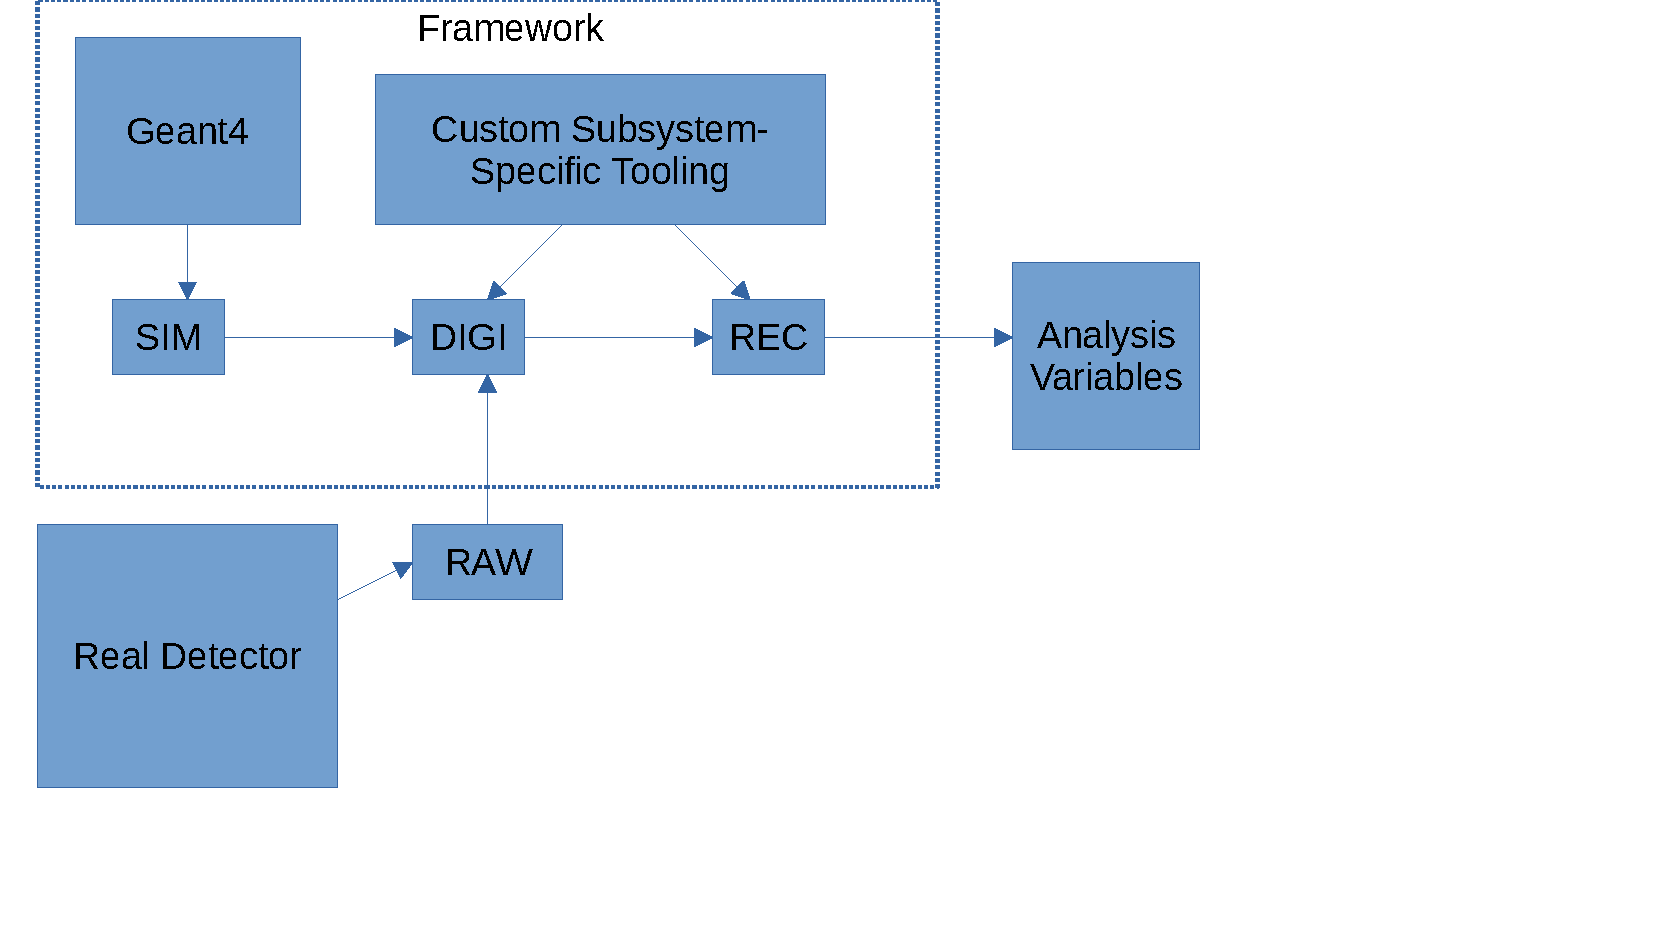
\includegraphics[width=0.9\textwidth]{figures/ldmx/simulation/data-flow.pdf}
  \caption{Diagram of processing stages within \ac{ldmx} showing the external sources of data or software that are used in those stages as well as which stages are commonly done within the centralized processing framework.}
  \label{fig:ldmx:sim:data-stages}
\end{figure}

In this work (as the chapter title implies), we focus mainly on the detector simulation stage where
data\todo[reword]{Distinguish ``data'' in software from the ``data'' of the experiment. What's
  another word for data that isn't overloaded?} is randomly generated in a way geared towards
realistically modeling the detector and particles interacting with it. The downstream stages,
namely electronic emulation and reconstruction, are not described further here; however, it should
be emphasized that all subsystems of \ac{ldmx} have their own custom implementations of these
stages in order to realistically emulate and reconstruct the data within their subsystem.

\subsection{Biasing and Filtering Technique}
Many of the processes most interesting for a \ac{dm} search within \ac{ldmx} are rare relative to
processes that are ``easier'' to reject by normal data processing.
In many cases, the rarity of these more interesting processes is a computational roadblock
since waiting for the entire detector simulation to complete before looking for these processes
of interest wastes a lot of computer time when only one out of every ten thousand events actually
contains a process we are interested in.
To make simulation of these processes more computationally feasible, we turn to the common simulation
techniques of biasing (artificially increasing the probability of a certain process occurring) and
filtering (ending the simulation of events if certain criteria are not met).

In the \ac{eat} analysis channel, all of our interesting processes occur within the developing
shower of particles in the \ac{ecal}.
While more complicated that checking for proceesses happening to the single beam electron,
we can enable looking for specific processes ocurring within this shower in a computationally
efficient way be tuning the order with which the simulation processes particles.
The detector simulation is focused only on particle-material interactions, so the order 
in which particles are simulated does not change how the physics is modeled.
We choose to process particles in two groups -- ``high'' and ``low'' energy --
where the high-energy particles are all processed before the low-energy particles.
The border between these two (called the ``Sorting Threshold'') is configurable by the user and enables a specific function\footnote{
The \texttt{NewStage} function of any \texttt{STACKING} \texttt{UserAction}s. 
} to be called mid-shower after all of the high-energy particles are processed
(i.e. simulated until their total energy falls below the Sorting Threshold).

Suppose we know from studying other (unbiased or low-bias) samples that showers need to have
a minimum amount of energy ``going into'' a specific process of interest before the shower
becomes ``important.''
We can set this minimum energy (here called the ``Filtering Threshold'') as a requirement on
the \ac{ecal} shower for the simulated event to be kept within the sample and, in order to
improve the speed of the filtering, we can apply this requirment \emph{during} the simulation
when the event transitions from the high-energy group to the low-energy group of particles.


Now, this infrastructure of determining a minimum simulated energy and having an energy-based
sorting of the processing order already helps improve the computational efficiency of these 
simluation samples (from $\sim 6$k CPU-hours to $\sim 30$ CPU-hours for $\sim 1$B EoT equivalent); 
nevertheless, it is still extremely slow and so we add biasing in order to artificially increase 
the rate of the process we wish the sample to focus on.
Since the processes we are interested in biasing are connected to particles that are abundant
within the electromagnetic \ac{ecal} shower, we need to require only particles above a
certain energy threshold (the ``Biasing Threshold'') to avoid over-sampling of the process.
In addition, we also need to define the factor that we will multiply the cross section by
when a particle is above the Biasing Threshold and in the \ac{ecal} volumes (the ``Biasing Factor'').

Artificially increasing the rate of a process relative to its true rate measured in nature
is obviously unphysical, but we can account for this by weighting the events depending on this
Biasing Factor when counting them.
The simulation engine we use does this weight calculation for us and it accounts for both the
biasing factor (beginning the weight with a factor of $1/B$) and unbiased processes happening
to a particle with biasing enabled (increasing the event weight to reflect that physical processes
at the natural rate have ocurred)

\begin{table}[htb]
    \centering
    \begin{tabular}{c|cc|p{0.4\textwidth}}
        Parameter & Dimension & Symbol & Short Description \\ \hline \hline
        Sorting Threshold & Energy & $T_S$ & Minimum total energy to be processed in first group \\ \hline
        Biasing Threshold & Energy & $T_B$ & Minimum total energy for a particle to be biased \\ \hline
        Biasing Factor & Dimension-less & $B$ & Factor to multiply cross section by \\ \hline
        Filtering Threshold & Energy & $T_F$ & Minimum energy transfered into a process for the event to be kept \\
    \end{tabular}
    \caption{Parameters of mid-shower biased samples. In all of the samples used in this study, we use the same value for the Sorting and Biasing Thresholds.}
    \label{tab:biasing-parameters}
\end{table}

Table \ref{tab:biasing-parameters} summarizes the parameters related to this
sample generation technique.
Practically, we choose to have the Biasing and Sorting Thresholds share the same value for all
of the samples in this work in order to reduce the number of parameters needed to tune and
to process all of the biased particles (as well as particles of similar energies
but different flavors) before making any filtering decision.

Generally, validation of this biasing and filtering technique can be done by checking that
the samples generated with this technique match samples generated without this technique
and with the filtering applied after the fact.
This validation needs to be done on a per-sample basis since the specific aspects of
the simulation that need to align may change depending on the specific physics
for which we are biasing and filtering.

\section{Standard Processes}
As displayed in \cref{fig:ldmx-bkgd-staircase}, there are a few categories of physics processes
that are described by the standard model and we expect to happen within our experiment. These
``background'' processes -- while interesting for other analyses of \ac{ldmx} data -- should be
rejected by this search for \ac{dm} since they are understood to \emph{not} be \ac{dm} by the
standard model and other experiments. In order to thoroughly and faithfully estimate our ability to
reject these backgrounds, we need to realistically simulate them within our detector volume.

\textsc{Geant4} \cite{geant4} has been developed for precisely this purpose. This study uses a slightly modified copy of \textsc{Geant4} v10.2.3 which focuses on improving the accuracy of processes relevant to a \ac{dm} search within \ac{ldmx} with the following needs.
\begin{enumerate}
  \item Updating cross section and sampling of $\gamma\to\mu^+\mu^-$ process to align it better with
        collected data and calculations of the standard model.
  \item Update nuclear cascade to align with more recent CLAS data specifically focused on the rate of
        low-multiplicity forward neutrons (Appendix A.A of \cite{ldmx-whitepaper}).
  \item Introduction of \emph{back scattering} $\pi^0$ in a $\gamma p \to \pi^0 p$ within a nuclear cascade
        (Appendix A.B of \cite{ldmx-whitepaper}).
\end{enumerate}
These updates enabled us to efficiently study the known and expected background processes interactions with the \ac{ldmx} detector design and compare this data to simulations of a model of a \ac{dm} production process.

\subsection{Dominate Contributors in this Analysis}
Generally, we focus on processes that would cause the energy in the \ac{ecal} to be
estimated at a significantly smaller value than the known beam energy.
This ``missing'' energy is used as a key piece of evidence that the event in question
should be stored for further study and thus is the main ingredient in the infrastructure
deciding whether a specific event should be stored (the ``trigger'').
From prior experience with \ac{ldmx} (e.g. \cite{ldmx-whitepaper,ldmx-photon-reject-2020}),
we expect certain types of standard processes to dominate the backgrounds that pass this
trigger requirement on missing energy: interactions with the nuclei of the detector
material producing hard-to-detect hadrons (so-called ``nuclear'' processes) and conversion
of photons into a pair of muons (which are also difficult for the \ac{ecal} to detect).

Nevertheless, we still can use a large, unbiased simulation sample in order to verify
these previous conclusions and inform our decisions on how the subsequent biased samples
should be produced.
\cref{fig:rec-efrac-by-nuc} is a key piece of evidence along these lines
where we separate the total reconstructed energy (the estimate from our detector)
as a fraction of the known beam energy by the amount of energy going into these nuclear
processes (so-called ``nuclear'' energy).
We see that as more energy is given to these nuclear interactions,
the reconstructed fraction decreases.
Eventually, we reach a point where enough energy has gone to these nuclear interactions
that we expect the event to be below the trigger threshold and be kept by the trigger
system at a significant rate.

\begin{figure}
  \centering
  \begin{tabular}{cc}
    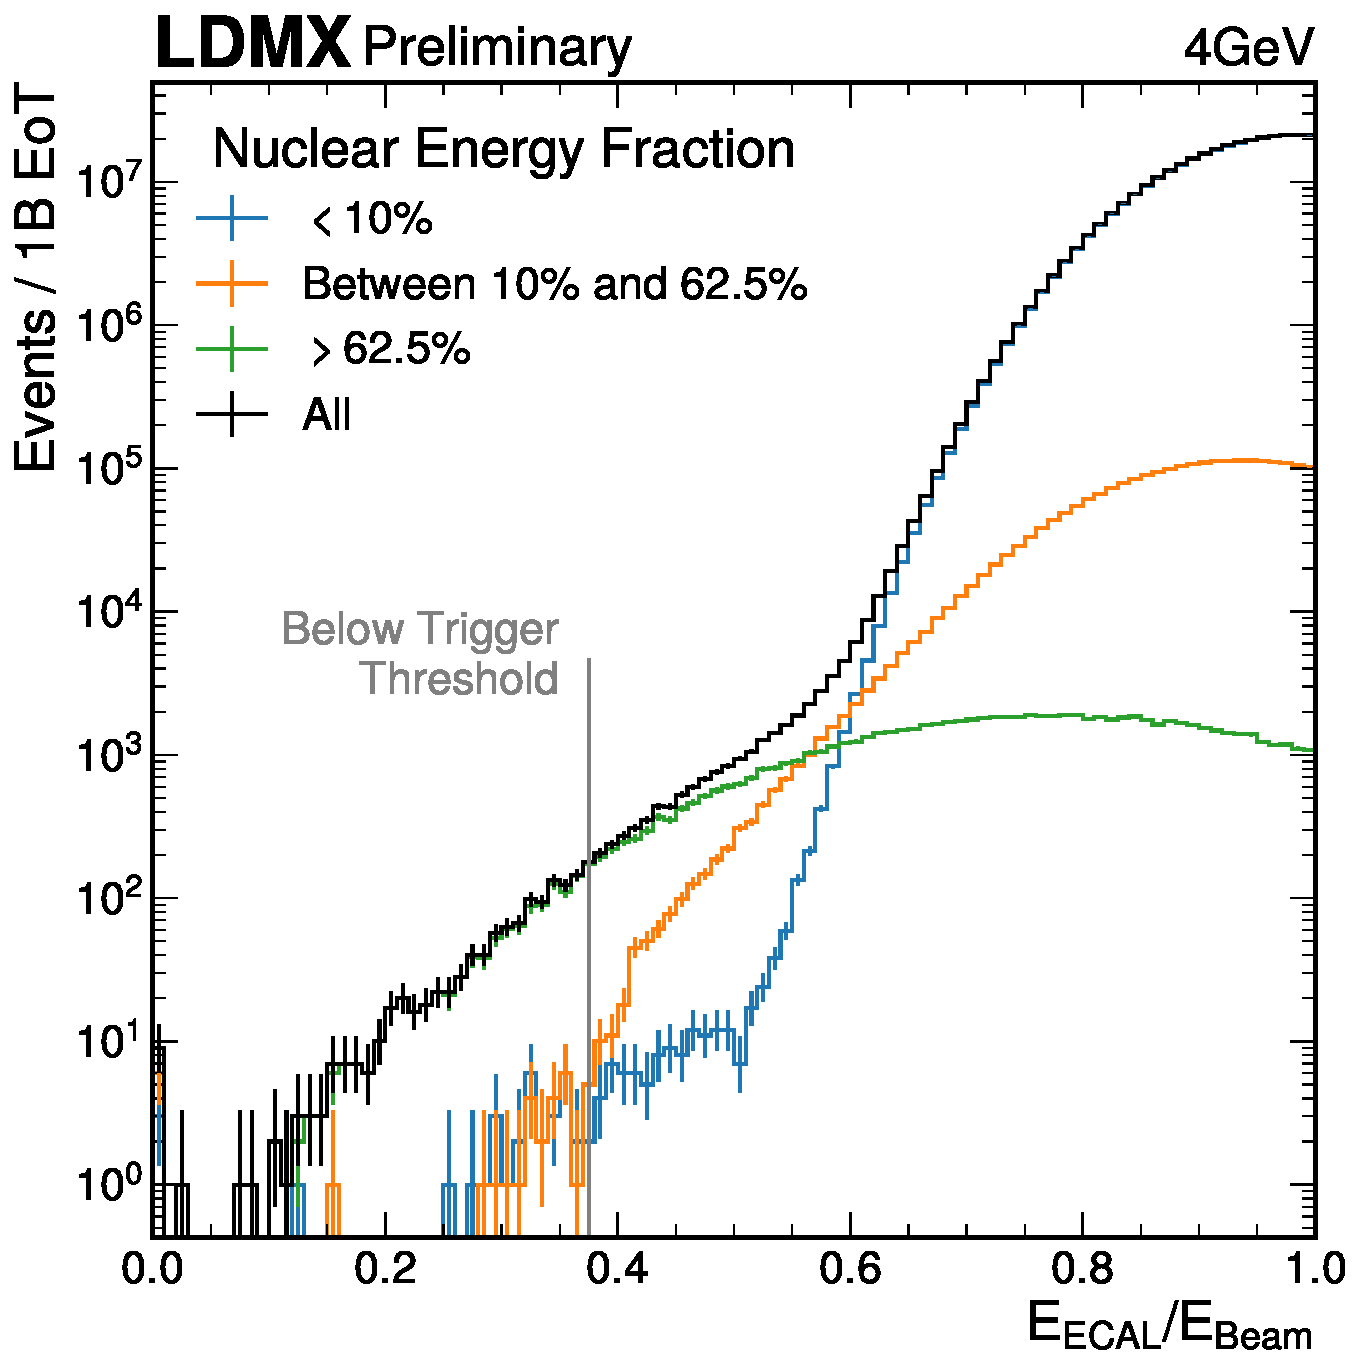
\includegraphics[width=0.49\textwidth]{figures/ldmx/simulation/4gev-ecal-by-nuc.pdf}
    &
    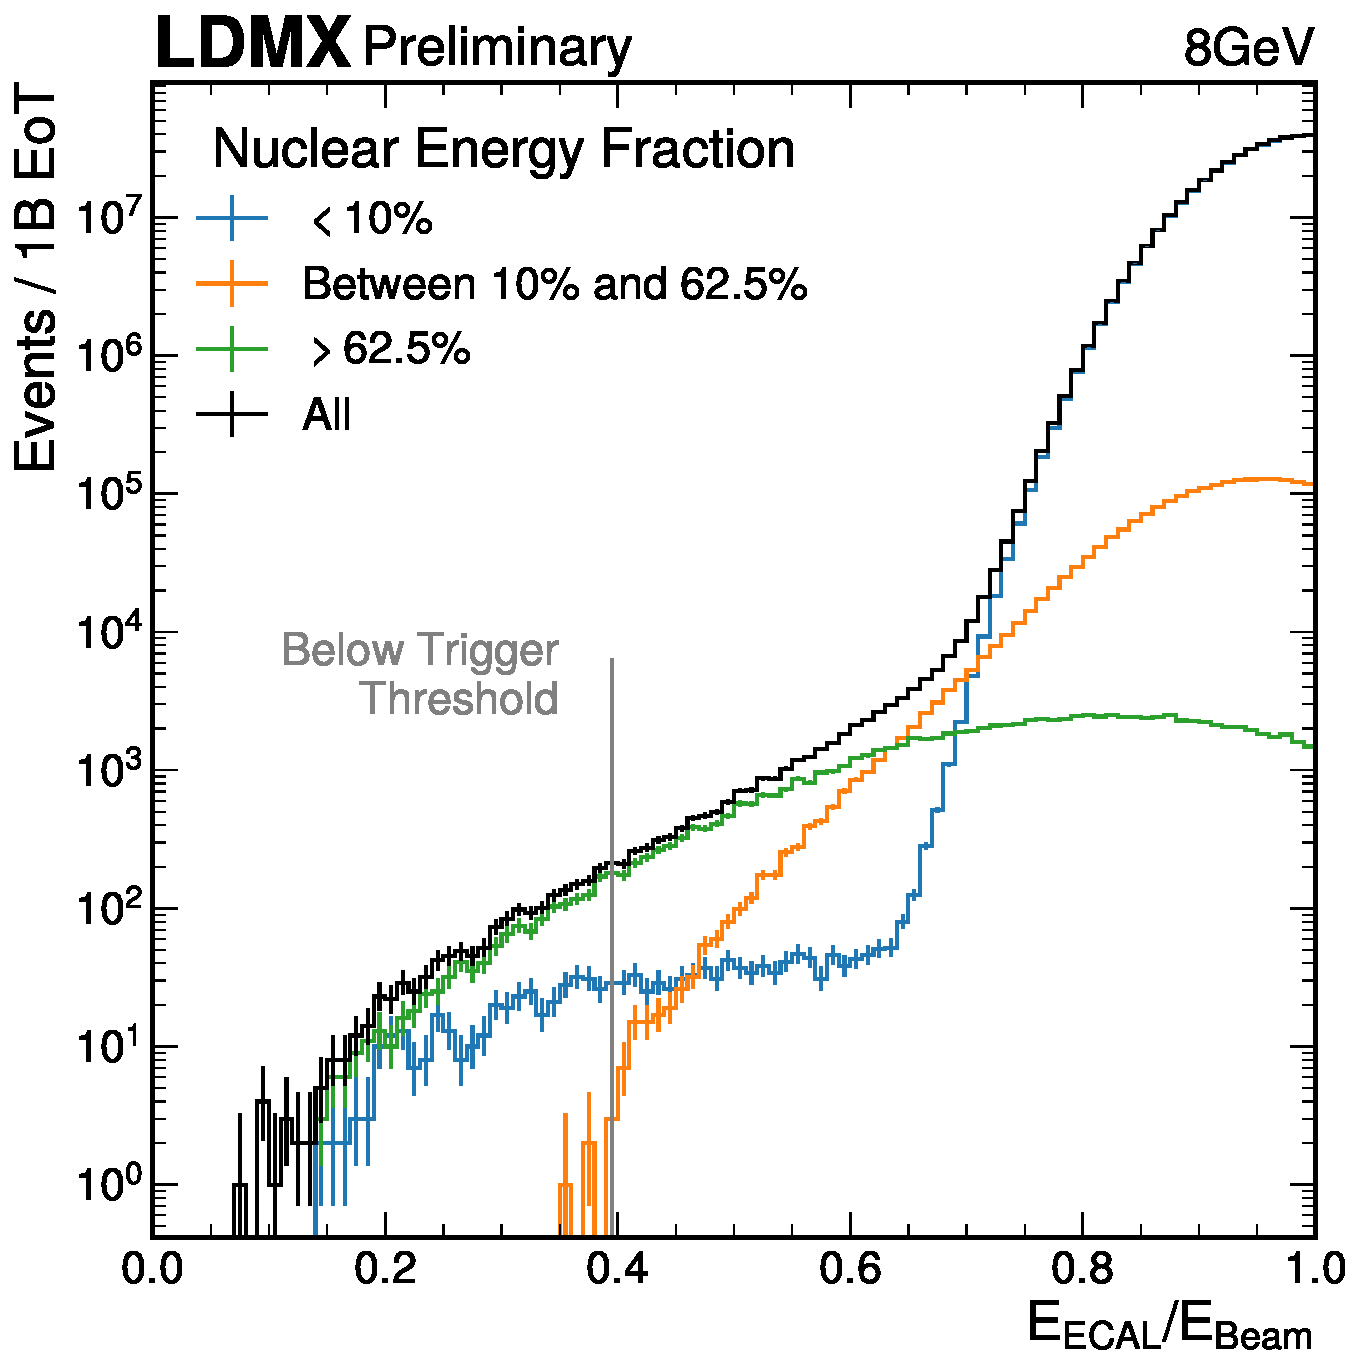
\includegraphics[width=0.49\textwidth]{figures/ldmx/simulation/8gev-ecal-by-nuc.pdf}
  \end{tabular}
  \caption{The total reconstructed energy within the \ac{ecal} as a fraction of the beam energy
  separated by the total nuclear energy within the event (the energy going into the photon-nuclear
  and electron-nuclear processes).}
  \label{fig:rec-efrac-by-nuc}
\end{figure}

\cref{fig:rec-efrac-by-nuc} shows that a significant fraction of events whose total nuclear
energy is greater than \qty{62.5}{\percent} of the beam energy fall below the threshold for
the trigger.
This figure also shows that there are other types of events that do not have much (if any)
nuclear interactions (since their nuclear energy is less than \qty{10}{\percent} of the beam
energy) but still are reconstructed below the trigger threshold.
\todo[dimuon]{insert dimuon plot to show that these other events are dimuon events}

\subsection{Expanding Production of these Processes}
\todo[copy]{Copy background sample validation appendices from EaT internal note.}

\section{Dark Matter Signal}
The particular signal process this analysis channel is looking for is the production of a dark
photon followed by an \emph{invisible} decay. In this regime, what happens to the dark photon after
it is produced is irrelevant to the analysis since both it and its products are not observable by
our detector.

With this focus in mind, we developed a dark bremsstrahlung simulation method that allows for the
visible particle (the recoiling lepton) to be distributed according to a full matrix element
calculation (via MG/ME) while the incident particle can have varied energy and be handled by Geant4
directly. This novel simulation technique allows for the dark bremsstrahlung process to be treated
(from Geant4's perspective) on the same footing as the background processes while maintaining the
precision of a matrix-calculator method.

\subsection{G4DarkBreM}
To accurately simulate the kinematics of the dark bremsstrahlung process for electrons in thick
targets, the process must be included at the level of experimental simulation instead of using
initial state event generators to account for the possibility of energy loss through bremsstrahlung
or multiple scattering prior to the dark matter interaction. Accurate kinematic simulation of the
outgoing electron are required for optimal experimental sensitivity measurements and appropriate
design of search strategies.

For this reason, we utilize G4DarkBreM \cite{g4darkbrem} which performs this embedding of the dark
bremmstrahlung process into \textsc{Geant}4. G4DarkBreM calculates the cross section using
numerical integrals of the Weizs\"{a}cker-Williams approximation, and the kinematics are simulated
using a scaling technique of \textsc{MadGraph/MadEvent} event libraries. The accuracy of the total
cross section and kinematics is validated using \textsc{MadGraph/MadEvent} samples at a range of
incident lepton energies.

\subsection{MadGraph/MadEvent}
For this study in \ac{ldmx}, the code package used to develop and validate G4DarkBreM was also used
to generate the input refernece libraries for sample generation. This code is a custom version of
\textsc{MadGraph/MadEvent4} with the following updates.
\begin{itemize}
  \item Introduction of basic dark sector particles (massive boson and spin-$1/2$ fermion) which act as the
        representatives of the dark sector interacting with the standard model particles.
  \item Definition of a nuclear particle (electrically neutral, spin-$1/2$ fermion) with new couplings to
        the dark photon including the nuclear form factors.
  \item Updating the definition of the electron to include its small (but non-zero) mass to prevent
        divergence of the cross section at lower energies.
\end{itemize}
These updates, along with some wrapping code, enables the generation of
dark bremmstrahlung events for a range of target nuclei, incident energies,
and either incident electrons or muons.

As suggested by the validation of G4DarkBreM \cite{g4darkbrem}, we generate libraries where the
incident electron's energy drops in steps of 10\% down from the beam energy. Since the dark photon
is required to be simulated with at least 50\% of the beam energy, we stop the library generation
also at 50\% of the beam energy. The primary nuclei that could dark brem within the \ac{ecal} are
tungsten, silicon, oxygen, and copper so those are the nuclei for which we generate libraries. The
rest of the nuclei within the simulated \ac{ecal} (sodium, calcium, carbon for example) have atomic
numbers close to those nuclei already sampled and so can be faithfully simulated with these
libraries. In order to avoid duplicating the same event, a unique reference library is generated
for each simulation run even when keeping the dark photon mass and beam energy the same.

\subsection{Characterization}
Describe how these samples "look"?

%%%%%%%%%%%%%%%%%%%%%%%%%%%%%%%%%%%%%%%%%%%%%%%%%%%%%%%%%%%%%%%%%%%%%%%%%%%%%%%%
